\chapter{Introdução}
\label{c.introducao}

“Com o advento da realidade virtual e o avanço dos recursos computacionais, as representações interativas e imersivas do imaginário, bem como a reprodução do real, tornaram-se mais fáceis de serem obtidas. ” (TORI; KIRNER; SISCOUTTO, 2006, p. 9).
A realidade virtual (RV) vem ganhando espaço em diversos setores como jogos, indústria e educação. Na área de jogos, empresas como Playstation® e Oculus® oferecem um acervo de jogos para as suas respectivas plataformas. Ao procurar por jogos em RV na Google Play, encontram-se algumas opções fornecidas por diversas empresas.
A realidade virtual pode ser utilizada na indústria para avaliar o design de um produto antes do mesmo ser produzido. A Ford Motor Company é uma das empresas que utilizam a realidade virtual. “O ‘Ford immersive Vehicle Environment (FiVE)’ é um sistema de realidade virtual altamente real e imersivo que aborda os desafios de design automotivo, engenharia e ergonomia.” (BARON, 2015, tradução nossa). Com esta tecnologia, é possível visualizar virtualmente tanto o exterior como o interior de um carro a ser produzido e avaliar aspectos de engenharia e design.
Já na área da educação, a realidade virtual pode ser aplicada através de jogos educativos e aulas imersivas. Imagine uma aula de história passada no local e no tempo de um acontecimento histórico, ou uma aula de astronomia no espaço. Pesquisas como Youngblut (1998) e Carvalho (2002) mostram como a realidade virtual pode ser incorporada na escola.
Para se obter uma experiência em realidade virtual, são necessários capacetes de visualização ou óculos de RV, um display por onde a aplicação irá rodar, um dispositivo de interação e a aplicação em RV. 
Atualmente existem vários modelos de óculos de RV com suporte à realidade virtual, tais como: Oculus Rift da Oculus® com preço estimado de R\$ 4.620,90 e Samsung Gear VR da Samsung® (R\$ 799,00). No entanto, o Google Cardboard da Google® é o que possui preço mais acessível em torno de R\$ 21,97 possuindo atualmente duas versões, cada uma com um meio de interação próprio. Em novembro 2016, a Google lança um novo visualizador denominado Daydream (Figura X). Este visualizador acompanha um controle com comunicação Bluetooth e o capacete de visualização feito com tecido para garantir maior conforto, além de um suporte para fixação do visualizador à cabeça do usuário. Atualmente, o único smartphone compatível com o Daydream é o Pixel, fabricado pela Google, pois o mesmo contém a última versão do sistema operacional Android: Android 7.0 Nougat.
As aplicações em RV podem ser desenvolvidas para plataformas mobile e desktop. A principal diferença entre as duas é a diferença de capacidade de processamento e memória, que são menores nos dispositivos móveis. Para as aplicações desktop utiliza-se óculos de RV como o Oculus Rift para rodar a aplicação. Já nas aplicações para dispositivos móveis, é necessário um visualizador como o Google Cardboard por onde o smartphone será encaixado.
A fim de interagir com o ambiente virtual, o usuário pode utilizar a movimentação da cabeça e um controle externo como luvas, mouse 3D, joystick, entre outros. “A necessidade de se fazer uso de aparatos tecnológicos para a interação do usuário com o ambiente virtual provoca restrições, tanto pelo aspecto econômico e tecnológico, quanto pelo desconforto, mas permite ao usuário fazer coisas que antes eram impossíveis ou inviáveis. ” (Tori, p.3)
Este projeto pretende utilizar óculos de RV e um dispositivo móvel para criar uma aplicação que utiliza os conceitos da realidade virtual visando explorar diferentes formas de controle de interação.

\section{Modificadores de Texto}
\label{s.modificador}

Os modificadores de texto mais simples utilizados são o negrito (``textbf'') \textbf{texto em negrito} e o itálico (``emph'') \emph{texto em itálico}.

\section{Seções}
\label{s.citacoes}

Seções podem ser criadas a partir do comando ``section'' e hierarquizadas abaixo do capítulo principal. É possível referenciá-las, por exemplo, Seção~\ref{s.citacoes} corresponde a seção atual em que estamos. Já se quisermos referenciar alguma outra coisa, é só utilizarmos o comando ``ref'' presente no código desse texto, por exemplo, Capítulo~\ref{c.introducao}.

\subsection{Subseções}
\label{ss.subsecao}

Subseções também podem ser criadas com o comando ``subsection'' e referenciadas~\ref{ss.subsecao}.

\subsubsection{Sub-subseções}
\label{sss.subsubsecao}

Também há mais um nível que pode ser criado com o comando ``subsubsection''.

\section{Alíneas}
\label{s.alineas}

\begin{alineas}

\item As alineas devem ser criadas desse modo, com o comando begin\{alineas\}. Isso é necessário para que estejam no formato definido pelo pacote abnTeX2 e, consequentemente, no formato definido pela ABNT.

\item Cada item da alínea pode ser invocado com um comando item.

\item O fim de cada alínea é determinado por end\{alineas\}.

\end{alineas}

\section{Tabelas}
\label{s.tabelas}

As tabelas também podem ser referenciadas como se fossem seções ou figuras, por exemplo, esta é a Tabela~\ref{t.transacao_mercado}.

\begin{table}[h]
\centering
\begin{tabular}{c|c}
\hline
\textbf{\small TID} & \textbf{\small Conjunto de Itens}\\\hline \hline
{\small 1} & {\small \{Pão, Leite\}}\\\hline
{\small 2} & {\small \{Pão, Fralda, Cerveja, Ovos\}}\\\hline
{\small 3} & {\small \{Leite, Fralda, Cerveja, Coca-Cola\}}\\\hline
{\small 4} & {\small \{Pão, Leite, Fralda, Cerveja\}}\\\hline
{\small 5} & {\small \{Pão, Leite, Fralda, Coca-Cola\}}\\\hline
\end{tabular}
\caption{Exemplo de transações de mercado.}
\label{t.transacao_mercado}
\end{table}

Quando uma tabela é criada com begin\{table\}, ela é automaticamente adicionada à Lista de Tabelas.

\section{Algoritmos}
\label{s.algoritmos}

O pacote nicealgo incluído nos arquivos desse projeto é responsável por disponibilizar comandos extras, não inerentes ao básico TeX, para a criação de algoritmos. Um exemplo do Algoritmo~\ref{a.algoritmo} é escrito a seguir. Eles também pode ser referenciados como se fossem tabelas ou figuras.

\begin{nicealgo}{a.algoritmo}
\naTITLE{Algoritmo AIS}
\naPREAMBLE
\naINPUT{Conjunto Frequente L = 0 e Grupo de Fronteira F = 0.}
\naBODY
\naBEGIN{\textbf{Enquanto} $F \neq 0$, \textbf{faça}}
\na{\textbf{Seja} conjunto candidato $C = 0$;}
\naBEGIN{\textbf{Para cada} tuplas $t$ da base de dados, \textbf{faça}}
\naBEGIN{\textbf{Para cada} conjuntos de itens $f$ em $F$, \textbf{faça}}
\naBEGIN{\textbf{Se} $t$ contém $f$, \textbf{então}}
\naEND{\textbf{Seja} $C_f =$ conjuntos de itens candidatos extensões de $f$ e contidos em $t$;}
\naBEGIN{\textbf{Para cada} conjunto de itens $c_f$ em $C_f$, \textbf{faça}}
\naBEGIN{\textbf{Se} $c_f \in C$, \textbf{então}}
\naEND{$c_f$.contagem $= c_f$.contagem$ + 1$;}
\naBEGIN{\textbf{Se não}}
\na{$c_f$.contagem $= 0$;}
\naEND{$C = C + c_f$;}
\naEND{}
\naEND{}
\naEND{}
\na{\textbf{Seja} F = 0;}
\naBEGIN{\textbf{Para cada} conjunto de itens $c$ em $C$, \textbf{faça}}
\naBEGIN{\textbf{Se} $contagem(c)/tamanho\_db > minsupport$, \textbf{então}}
\naEND{$L = L + c$;}
\naBEGIN{\textbf{Se} $c$ deve ser usado como a próxima fronteira, \textbf{então}}
\naEND{$F = F + c$;}
\naEND{}
\naEND{}
\end{nicealgo}

\section{Figuras}
\label{s.figuras}

Abaixo podemos identificar a criação e referência da Figura~\ref{f.disposicao_mercado}. Atente-se ao código para perceber um possível redimensionamento com a função scale e o caminho de onde a figura deve ser retirada.

Quando uma figura é criada com begin\{figure\}, ela é automaticamente adicionada à Lista de Ilustrações.

\begin{figure}[h]
\caption{\small Exemplo do ambiente TeXworks.}
\centering
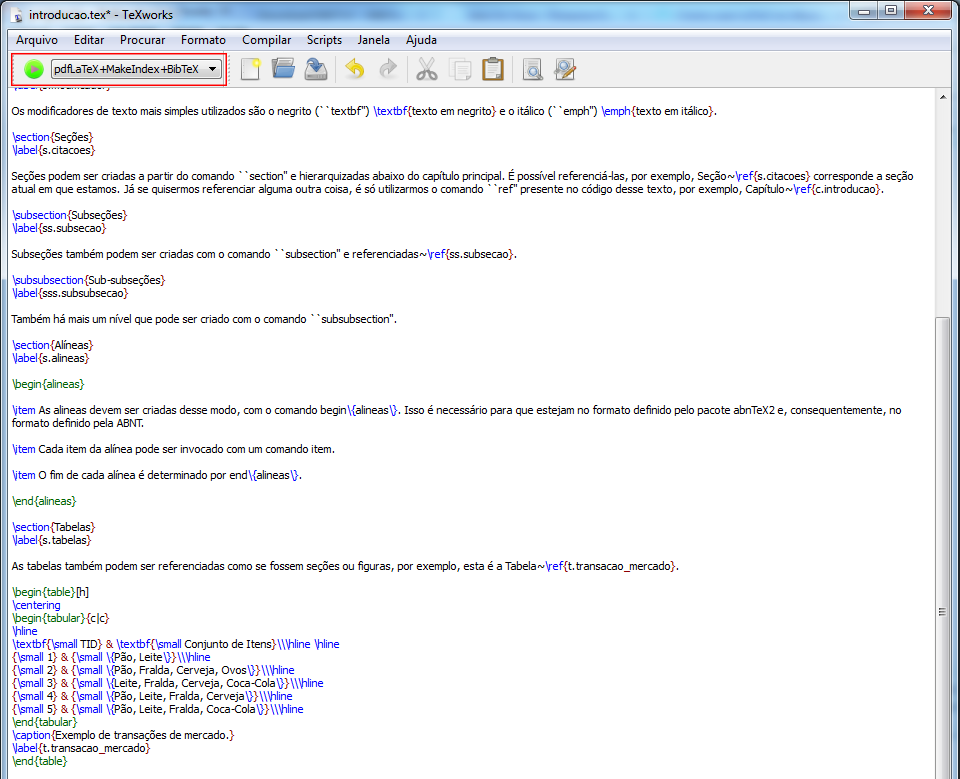
\includegraphics[scale=0.50]{figs/tex_exemplo.png}
\label{f.disposicao_mercado}
\legend{\small Fonte: Elaborada pelo autor.}
\end{figure}

\section{Equações}
\label{s.equacoes}

O TeX também é muito famoso pela forma em que consegue tratar funções e símbolos matemáticos. A partir da utiização de dois cifrões (\$codigo matemático\$) é possível identificar ao compilador que a escrita a seguir são símbolos e códigos originários do pacote matemático do TeX. Aqui estamos demonstrado um exemplo $\phi = 1 + x$ dessa utilização.

Também podemos definir equações utilizando os comandos begin\{equation\} e end\{equation\}. Por exemplo:

\begin{equation}
\label{e.energy_rbm}
E(\textbf{v},\textbf{h})=-\sum_{i=1}^ma_iv_i-\sum_{j=1}^nb_jh_j-\sum_{i=1}^m\sum_{j=1}^nv_ih_jw_{ij},
\end{equation}

\begin{equation}
\label{e.probability_configuration}
P(\textbf{v},\textbf{h})=\frac{e^{-E(\textbf{v},\textbf{h})}}{\displaystyle\sum_{\textbf{v},\textbf{h}}e^{-E(\textbf{v},\textbf{h})}},
\end{equation}

\begin{eqnarray}
\label{eq:par}
\hat{\phi}^j & = & \left\{ \begin{array}{ll} \hat{\phi}^j\pm \varphi_j \varrho  & \mbox{{ com probabilidade PAR}} \\
    \hat{\phi}^j & \mbox{{com probabilidade (1-PAR).}}
\end{array}\right.
\end{eqnarray}

Existem diversos sites no Google que contém códigos de símbolos e funções matemáticas de todos os tipos. Exemplo:\\
\begin{center}
\tiny estudijas.lu.lv/pluginfile.php/14809/mod\_page/content/16/instrukcijas/matematika\_moodle/LaTeX\_Symbols.pdf.
\end{center}

\section{Como citar as referências}
\label{ss.referencias}

Aqui está um exemplo de como podemos referenciar as bibliografias utilizadas no trabalho. Elas são guardadas na forma de metadados (tags) no arquivo .bib a qual é importada no projeto principal (projeto.tex).

E podemos citá-las de acordo com os identificadores atribuídos para cada referência, por exemplo,~\cite{stonebraker93} e~\cite{rocha09}.

Após citar um item de referência bibliográfica com o comando ``cite'', ela será automaticamente padronizada e incluída na página de Referências de seu arquivo. Atualmente os maiores sites portadores de artigos, periódicos, dentre outros (IEEE, Springer, etc) já conseguem exportar a publicação desejado no formato BibTeX, sendo facilmente adicionado ao arquivo .bib de seu trabalho.


chapter{Introdução}
\label{c.introducao}

“Com o advento da realidade virtual e o avanço dos recursos computacionais, as representações interativas e imersivas do imaginário, bem como a reprodução do real, tornaram-se mais fáceis de serem obtidas. ” (TORI; KIRNER; SISCOUTTO, 2006, p. 9).
A realidade virtual (RV) vem ganhando espaço em diversos setores como jogos, indústria e educação. Na área de jogos, empresas como Playstation® e Oculus® oferecem um acervo de jogos para as suas respectivas plataformas. Ao procurar por jogos em RV na Google Play, encontram-se algumas opções fornecidas por diversas empresas.
A realidade virtual pode ser utilizada na indústria para avaliar o design de um produto antes do mesmo ser produzido. A Ford Motor Company é uma das empresas que utilizam a realidade virtual. “O ‘Ford immersive Vehicle Environment (FiVE)’ é um sistema de realidade virtual altamente real e imersivo que aborda os desafios de design automotivo, engenharia e ergonomia.” (BARON, 2015, tradução nossa). Com esta tecnologia, é possível visualizar virtualmente tanto o exterior como o interior de um carro a ser produzido e avaliar aspectos de engenharia e design.
Já na área da educação, a realidade virtual pode ser aplicada através de jogos educativos e aulas imersivas. Imagine uma aula de história passada no local e no tempo de um acontecimento histórico, ou uma aula de astronomia no espaço. Pesquisas como Youngblut (1998) e Carvalho (2002) mostram como a realidade virtual pode ser incorporada na escola.
Para se obter uma experiência em realidade virtual, são necessários capacetes de visualização ou óculos de RV, um display por onde a aplicação irá rodar, um dispositivo de interação e a aplicação em RV. 
Atualmente existem vários modelos de óculos de RV com suporte à realidade virtual, tais como: Oculus Rift da Oculus® com preço estimado de R\$ 4.620,90 e Samsung Gear VR da Samsung® (R\$ 799,00). No entanto, o Google Cardboard da Google® é o que possui preço mais acessível em torno de R\$ 21,97 possuindo atualmente duas versões, cada uma com um meio de interação próprio. Em novembro 2016, a Google lança um novo visualizador denominado Daydream (Figura X). Este visualizador acompanha um controle com comunicação Bluetooth e o capacete de visualização feito com tecido para garantir maior conforto, além de um suporte para fixação do visualizador à cabeça do usuário. Atualmente, o único smartphone compatível com o Daydream é o Pixel, fabricado pela Google, pois o mesmo contém a última versão do sistema operacional Android: Android 7.0 Nougat.
As aplicações em RV podem ser desenvolvidas para plataformas mobile e desktop. A principal diferença entre as duas é a diferença de capacidade de processamento e memória, que são menores nos dispositivos móveis. Para as aplicações desktop utiliza-se óculos de RV como o Oculus Rift para rodar a aplicação. Já nas aplicações para dispositivos móveis, é necessário um visualizador como o Google Cardboard por onde o smartphone será encaixado.
A fim de interagir com o ambiente virtual, o usuário pode utilizar a movimentação da cabeça e um controle externo como luvas, mouse 3D, joystick, entre outros. “A necessidade de se fazer uso de aparatos tecnológicos para a interação do usuário com o ambiente virtual provoca restrições, tanto pelo aspecto econômico e tecnológico, quanto pelo desconforto, mas permite ao usuário fazer coisas que antes eram impossíveis ou inviáveis. ” (Tori, p.3)
Este projeto pretende utilizar óculos de RV e um dispositivo móvel para criar uma aplicação que utiliza os conceitos da realidade virtual visando explorar diferentes formas de controle de interação.

\section{Modificadores de Texto}
\label{s.modificador}

Os modificadores de texto mais simples utilizados são o negrito (``textbf'') \textbf{texto em negrito} e o itálico (``emph'') \emph{texto em itálico}.

\section{Seções}
\label{s.citacoes}

Seções podem ser criadas a partir do comando ``section'' e hierarquizadas abaixo do capítulo principal. É possível referenciá-las, por exemplo, Seção~\ref{s.citacoes} corresponde a seção atual em que estamos. Já se quisermos referenciar alguma outra coisa, é só utilizarmos o comando ``ref'' presente no código desse texto, por exemplo, Capítulo~\ref{c.introducao}.

\subsection{Subseções}
\label{ss.subsecao}

Subseções também podem ser criadas com o comando ``subsection'' e referenciadas~\ref{ss.subsecao}.

\subsubsection{Sub-subseções}
\label{sss.subsubsecao}

Também há mais um nível que pode ser criado com o comando ``subsubsection''.

\section{Alíneas}
\label{s.alineas}

\begin{alineas}
	
	\item As alineas devem ser criadas desse modo, com o comando begin\{alineas\}. Isso é necessário para que estejam no formato definido pelo pacote abnTeX2 e, consequentemente, no formato definido pela ABNT.
	
	\item Cada item da alínea pode ser invocado com um comando item.
	
	\item O fim de cada alínea é determinado por end\{alineas\}.
	
\end{alineas}

\section{Tabelas}
\label{s.tabelas}

As tabelas também podem ser referenciadas como se fossem seções ou figuras, por exemplo, esta é a Tabela~\ref{t.transacao_mercado}.

\begin{table}[h]
	\centering
	\begin{tabular}{c|c}
		\hline
		\textbf{\small TID} & \textbf{\small Conjunto de Itens}\\\hline \hline
		{\small 1} & {\small \{Pão, Leite\}}\\\hline
		{\small 2} & {\small \{Pão, Fralda, Cerveja, Ovos\}}\\\hline
		{\small 3} & {\small \{Leite, Fralda, Cerveja, Coca-Cola\}}\\\hline
		{\small 4} & {\small \{Pão, Leite, Fralda, Cerveja\}}\\\hline
		{\small 5} & {\small \{Pão, Leite, Fralda, Coca-Cola\}}\\\hline
	\end{tabular}
	\caption{Exemplo de transações de mercado.}
	\label{t.transacao_mercado}
\end{table}

Quando uma tabela é criada com begin\{table\}, ela é automaticamente adicionada à Lista de Tabelas.

\section{Algoritmos}
\label{s.algoritmos}

O pacote nicealgo incluído nos arquivos desse projeto é responsável por disponibilizar comandos extras, não inerentes ao básico TeX, para a criação de algoritmos. Um exemplo do Algoritmo~\ref{a.algoritmo} é escrito a seguir. Eles também pode ser referenciados como se fossem tabelas ou figuras.

\begin{nicealgo}{a.algoritmo}
	\naTITLE{Algoritmo AIS}
	\naPREAMBLE
	\naINPUT{Conjunto Frequente L = 0 e Grupo de Fronteira F = 0.}
	\naBODY
	\naBEGIN{\textbf{Enquanto} $F \neq 0$, \textbf{faça}}
	\na{\textbf{Seja} conjunto candidato $C = 0$;}
	\naBEGIN{\textbf{Para cada} tuplas $t$ da base de dados, \textbf{faça}}
	\naBEGIN{\textbf{Para cada} conjuntos de itens $f$ em $F$, \textbf{faça}}
	\naBEGIN{\textbf{Se} $t$ contém $f$, \textbf{então}}
	\naEND{\textbf{Seja} $C_f =$ conjuntos de itens candidatos extensões de $f$ e contidos em $t$;}
	\naBEGIN{\textbf{Para cada} conjunto de itens $c_f$ em $C_f$, \textbf{faça}}
	\naBEGIN{\textbf{Se} $c_f \in C$, \textbf{então}}
	\naEND{$c_f$.contagem $= c_f$.contagem$ + 1$;}
	\naBEGIN{\textbf{Se não}}
	\na{$c_f$.contagem $= 0$;}
	\naEND{$C = C + c_f$;}
	\naEND{}
	\naEND{}
	\naEND{}
	\na{\textbf{Seja} F = 0;}
	\naBEGIN{\textbf{Para cada} conjunto de itens $c$ em $C$, \textbf{faça}}
	\naBEGIN{\textbf{Se} $contagem(c)/tamanho\_db > minsupport$, \textbf{então}}
	\naEND{$L = L + c$;}
	\naBEGIN{\textbf{Se} $c$ deve ser usado como a próxima fronteira, \textbf{então}}
	\naEND{$F = F + c$;}
	\naEND{}
	\naEND{}
\end{nicealgo}

\section{Figuras}
\label{s.figuras}

Abaixo podemos identificar a criação e referência da Figura~\ref{f.disposicao_mercado}. Atente-se ao código para perceber um possível redimensionamento com a função scale e o caminho de onde a figura deve ser retirada.

Quando uma figura é criada com begin\{figure\}, ela é automaticamente adicionada à Lista de Ilustrações.

\begin{figure}[h]
	\caption{\small Exemplo do ambiente TeXworks.}
	\centering
	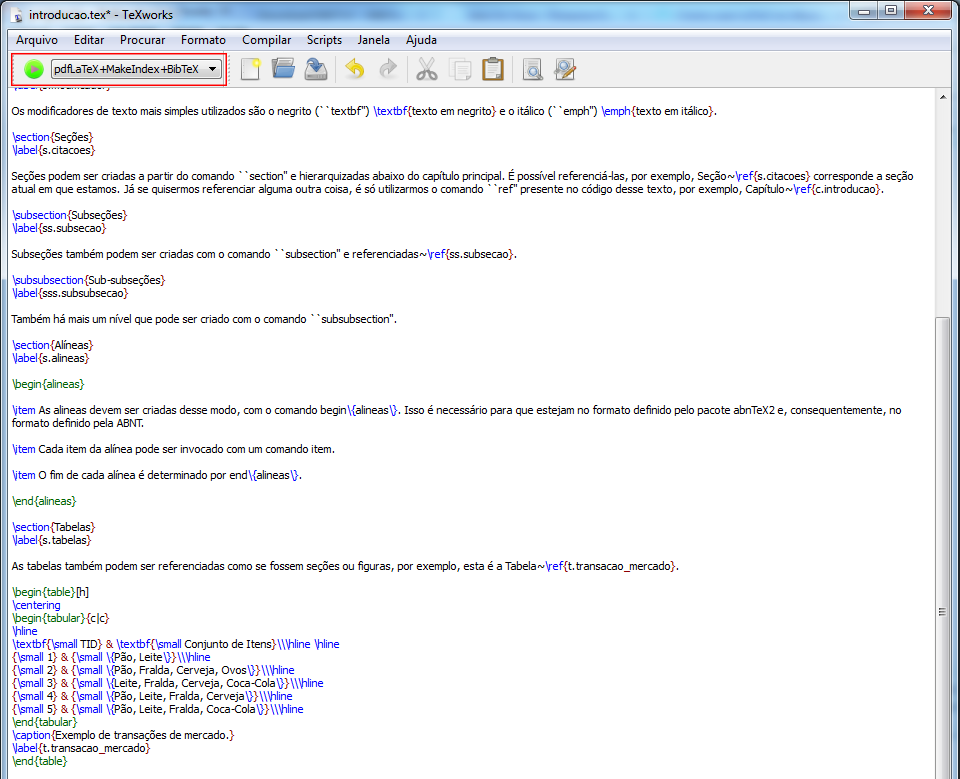
\includegraphics[scale=0.50]{figs/tex_exemplo.png}
	\label{f.disposicao_mercado}
	\legend{\small Fonte: Elaborada pelo autor.}
\end{figure}

\section{Equações}
\label{s.equacoes}

O TeX também é muito famoso pela forma em que consegue tratar funções e símbolos matemáticos. A partir da utiização de dois cifrões (\$codigo matemático\$) é possível identificar ao compilador que a escrita a seguir são símbolos e códigos originários do pacote matemático do TeX. Aqui estamos demonstrado um exemplo $\phi = 1 + x$ dessa utilização.

Também podemos definir equações utilizando os comandos begin\{equation\} e end\{equation\}. Por exemplo:

\begin{equation}
\label{e.energy_rbm}
E(\textbf{v},\textbf{h})=-\sum_{i=1}^ma_iv_i-\sum_{j=1}^nb_jh_j-\sum_{i=1}^m\sum_{j=1}^nv_ih_jw_{ij},
\end{equation}

\begin{equation}
\label{e.probability_configuration}
P(\textbf{v},\textbf{h})=\frac{e^{-E(\textbf{v},\textbf{h})}}{\displaystyle\sum_{\textbf{v},\textbf{h}}e^{-E(\textbf{v},\textbf{h})}},
\end{equation}

\begin{eqnarray}
\label{eq:par}
\hat{\phi}^j & = & \left\{ \begin{array}{ll} \hat{\phi}^j\pm \varphi_j \varrho  & \mbox{{ com probabilidade PAR}} \\
\hat{\phi}^j & \mbox{{com probabilidade (1-PAR).}}
\end{array}\right.
\end{eqnarray}

Existem diversos sites no Google que contém códigos de símbolos e funções matemáticas de todos os tipos. Exemplo:\\
\begin{center}
	\tiny estudijas.lu.lv/pluginfile.php/14809/mod\_page/content/16/instrukcijas/matematika\_moodle/LaTeX\_Symbols.pdf.
\end{center}

\section{Como citar as referências}
\label{ss.referencias}

Aqui está um exemplo de como podemos referenciar as bibliografias utilizadas no trabalho. Elas são guardadas na forma de metadados (tags) no arquivo .bib a qual é importada no projeto principal (projeto.tex).

E podemos citá-las de acordo com os identificadores atribuídos para cada referência, por exemplo,~\cite{stonebraker93} e~\cite{rocha09}.

Após citar um item de referência bibliográfica com o comando ``cite'', ela será automaticamente padronizada e incluída na página de Referências de seu arquivo. Atualmente os maiores sites portadores de artigos, periódicos, dentre outros (IEEE, Springer, etc) já conseguem exportar a publicação desejado no formato BibTeX, sendo facilmente adicionado ao arquivo .bib de seu trabalho.

